\documentclass{article}
\iffalse
This file is protected by Copyright. Please refer to the COPYRIGHT file
distributed with this source distribution.

This file is part of OpenCPI <http://www.opencpi.org>

OpenCPI is free software: you can redistribute it and/or modify it under the
terms of the GNU Lesser General Public License as published by the Free Software
Foundation, either version 3 of the License, or (at your option) any later
version.

OpenCPI is distributed in the hope that it will be useful, but WITHOUT ANY
WARRANTY; without even the implied warranty of MERCHANTABILITY or FITNESS FOR A
PARTICULAR PURPOSE. See the GNU Lesser General Public License for more details.

You should have received a copy of the GNU Lesser General Public License along
with this program. If not, see <http://www.gnu.org/licenses/>.
\fi

\author{} % Force author to be blank
%----------------------------------------------------------------------------------------
% Paper size, orientation and margins
%----------------------------------------------------------------------------------------
\usepackage{geometry}
\geometry{
	letterpaper,			% paper type
	portrait,				% text direction
	left=.75in,				% left margin
	top=.75in,				% top margin
	right=.75in,			% right margin
	bottom=.75in			% bottom margin
 }
%----------------------------------------------------------------------------------------
% Header/Footer
%----------------------------------------------------------------------------------------
\usepackage{fancyhdr} \pagestyle{fancy} % required for fancy headers
\renewcommand{\headrulewidth}{0.5pt}
\renewcommand{\footrulewidth}{0.5pt}
\rhead{\small{ANGRYVIPER Team}}
%----------------------------------------------------------------------------------------
% Appendix packages
%----------------------------------------------------------------------------------------
\usepackage[toc,page]{appendix}
%----------------------------------------------------------------------------------------
% Defined Commands & Renamed Commands
%----------------------------------------------------------------------------------------
\renewcommand{\contentsname}{Table of Contents}
\renewcommand{\listfigurename}{List of Figures}
\renewcommand{\listtablename}{List of Tables}
\newcommand{\todo}[1]{\textcolor{red}{TODO: #1}\PackageWarning{TODO:}{#1}} % To do notes
\newcommand{\code}[1]{\texttt{#1}} % For inline code snippet or command line
%----------------------------------------------------------------------------------------
% Various pacakges
%----------------------------------------------------------------------------------------
\usepackage{hyperref} % for linking urls and lists
\usepackage{graphicx} % for including pictures by file
\usepackage{listings} % for coding language styles
\usepackage{rotating} % for sideways table
\usepackage{pifont}   % for sideways table
\usepackage{pdflscape} % for landscape view
%----------------------------------------------------------------------------------------
% Table packages
%----------------------------------------------------------------------------------------
\usepackage{longtable} % for long possibly multi-page tables
\usepackage{tabularx} % c=center,l=left,r=right,X=fill
\usepackage{float}
\floatstyle{plaintop}
\usepackage[tableposition=top]{caption}
\newcolumntype{P}[1]{>{\centering\arraybackslash}p{#1}}
\newcolumntype{M}[1]{>{\centering\arraybackslash}m{#1}}
%----------------------------------------------------------------------------------------
% Block Diagram / FSM Drawings
%----------------------------------------------------------------------------------------
\usepackage{tikz}
\usetikzlibrary{shapes,arrows,fit,positioning}
\usetikzlibrary{automata} % used for the fsm
%----------------------------------------------------------------------------------------
% Colors Used
%----------------------------------------------------------------------------------------
\usepackage{colortbl}
\definecolor{blue}{rgb}{.7,.8,.9}
\definecolor{ceruleanblue}{rgb}{0.16, 0.32, 0.75}
\definecolor{drkgreen}{rgb}{0,0.6,0}
\definecolor{deepmagenta}{rgb}{0.8, 0.0, 0.8}
\definecolor{cyan}{rgb}{0.0,0.6,0.6}
\definecolor{maroon}{rgb}{0.5,0,0}
%----------------------------------------------------------------------------------------
% Update the docTitle and docVersion per document
%----------------------------------------------------------------------------------------
\def\docTitle{Component Data Sheet}
\def\docVersion{1.5}
%----------------------------------------------------------------------------------------
\date{Version \docVersion} % Force date to be blank and override date with version
\title{\docTitle}
\lhead{\small{\docTitle}}

\def\comp{baudtracking\_simple}
\edef\ecomp{baudtracking_simple}
\def\Comp{Baud Tracking Simple}
\graphicspath{ {figures/} }

\begin{document}

\section*{Summary - \Comp}
\begin{tabular}{|c|M{13.5cm}|}
	\hline
	\rowcolor{blue}
	                  &                                          \\
	\hline
	Name              & \comp                                    \\
	\hline
	Worker Type       & Application                              \\
	\hline
	Version           & v\docVersion \\
	\hline
	Release Date      & 4/2019 \\
	\hline
	Component Library & ocpi.assets.dsp\_comps                    \\
	\hline
	Workers           & \comp.rcc                                \\
	\hline
	Tested Platforms  & centos7, xilinx13\_3, xilinx13\_4 \\
	\hline
\end{tabular}
\section*{Worker Implementation Details}
\subsection*{\comp.rcc}
\begin{flushleft}
	The input data to this worker is expected to be pulse shaped samples.  The full length of the baud in samples (SPB) is averaged over BaudAvrCount bauds.  The maximum of this array of averages is then calculated, if this is not in the mid point of the array, then a drift is calculated.  The midpoint of the next SPB envelope is then shifted based on the drift value.\par\medskip

	\begin{figure}[h]
		\centering
		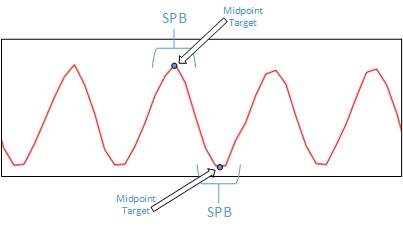
\includegraphics[scale=.75]{baudtracker_signal}
		\caption{Functionality Diagram}
		\label{fig:sig}
	\end{figure}

	For a consistent signal, the algorithm will lock on after a few iterations followed by a few small adjustments. If you are not exactly sure of the SPB, the algorithm will constantly adjust and find the peak values as long as the SPB is not off by too much.
\end{flushleft}

\section*{Block Diagrams}
\subsection*{Top level}
\begin{center}
	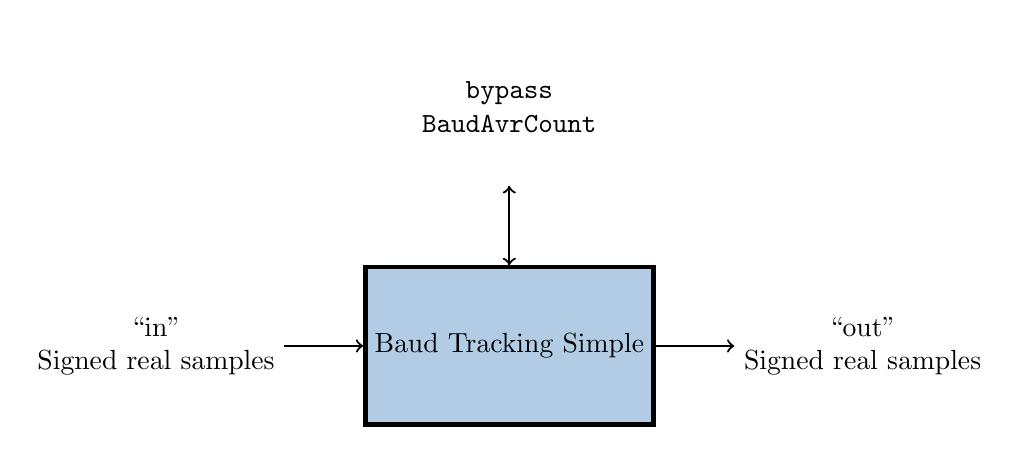
\begin{tikzpicture}[% List of styles applied to all, to override specify on a case-by-case
			every node/.style={
				align=center,  		% use this so that the "\\" for line break works
				minimum size=2cm	% creates space above and below text in rectangle
			},
			every edge/.style={draw,thick}
		]
		\node[rectangle,ultra thick,draw=black,fill=blue](R2){\Comp};
		\node[rectangle,draw=white,fill=white](R3)[left= of R2]{``in'' \\ Signed real samples};
		\node[rectangle,draw=white,fill=white](R4)[right= of R2]{``out'' \\ Signed real samples};
		\node[rectangle,draw=white,fill=white](R5)[above= of R2]{\verb+bypass+\\ \verb+BaudAvrCount+};
		\path[->]
		(R3)edge []	node [] {} (R2)
		(R2)edge []	node [] {} (R4)
		(R2)edge []	node [] {} (R5)
		(R5)edge []	node [] {} (R2)
		;
	\end{tikzpicture}
\end{center}

\section*{Source Dependencies}
\subsection*{\comp.rcc}
\begin{itemize}
	\item ocpi.assets/components/dsp\_comps/Baudtracking\_simple.rcc/Baudtracking\_simple.c
\end{itemize}

\begin{landscape}
	\section*{Component Spec Properties}
	\begin{scriptsize}
		\begin{tabular}{|p{3cm}|p{1.5cm}|c|c|c|c|c|p{7cm}|}
			\hline
			\rowcolor{blue}
			Name                & Type  & SequenceLength & ArrayDimensions & Accessibility      & Valid Range & Default & Usage                                                                                                                                                                                                                                                                                            \\
			\hline
			\verb+bypass+       & Bool  & -              & -               & Readable, Writable & Standard    & -       & When set to true the worker will pass its input to its output without any processing.  False means normal operation.                                                                                                                                                                             \\
			\hline
			\verb+BaudAvrCount+ & Short & -              & -               & Readable, Writable & 5-34767     & -       & The number of bauds to average over to determine drift(10 is a good place to start).  If this number is too high the algorithm won't be able to compensate quickly enough if the average number is too low it will adjust back and forth without enough averages to make an intelligent decision. \\
			\hline
		\end{tabular}
	\end{scriptsize}
	\section*{Worker Properties}
	\subsection*{\comp.rcc}
	Control Operations: Start\newline\newline
	\begin{scriptsize}
		\begin{tabular}{|p{3cm}|p{2cm}|p{1cm}|c|c|c|c|c|p{5cm}|}
			\hline
			\rowcolor{blue}
			Type     & Name       & Type   & SequenceLength & ArrayDimensions & Accessibility     & Valid Range & Default & Usage                                                                                                                                                                             \\
			\hline
			Property & \verb+SPB+ & UShort & -              & -               & Readable,Writable & 3-100       & 5       & The expected number of samples per baud.  This number can be slightly off and the algorithm will work correctly. As long as it is close, the averaging mechanism will compensate. \\
			\hline
		\end{tabular}
	\end{scriptsize}

	\section*{Component Ports}
	\begin{scriptsize}
		\begin{tabular}{|M{2cm}|M{1.5cm}|M{4cm}|c|c|M{9cm}|}
			\hline
			\rowcolor{blue}
			Name & Producer & Protocol          & Optional & Advanced & Usage               \\
			\hline
			in   & false    & rstream\_protocol & false    & -        & Signed real samples \\
			\hline
			out  & true     & rstream\_protocol & false    & -        & Signed real samples \\
			\hline
		\end{tabular}
	\end{scriptsize}
\end{landscape}

\begin{landscape}
\section*{Performance and Resource Utilization}
\subsubsection*{\comp.rcc}
\begin{scriptsize}
	\begin{tabular}{|c|c|c|}
		\hline
		\rowcolor{blue}
		Processor Type & Processor Frequency & Run Function Time \\
		\hline
		TBD            & TBD                 & TBD               \\
		\hline
	\end{tabular}
\end{scriptsize}
\end{landscape}

\section*{Test and Verification}
\begin{flushleft}
	No unit test currently exists for this worker.
\end{flushleft}
\end{document}
